\section{薛定谔方程}

\begin{quotation}
``自然科学不是自然本身,而是人和自然关系的一部分,因而就依赖于人。''\qquad 海森堡
\end{quotation}

一个微观粒子的运动状态可以用波函数$\psi $来描述,
有了波函数就可求得物理量的期望值,
并与测量值进行比较。现在还需要一个描述波函数如何随时间演化的波动方程(wave
equation),
以及如何由已知条件求解波函数。我们可以先回顾一下经典的波动方程:$\frac{\partial^2
u}{\partial t^2} = c^2 \nabla^2
u$;和经典的电磁波波动方程\footnote{为什么光子的波动性很容易被观察到,
而电子的波动性不容易被观察到,这是由于光子是无相互作用Bose子,
可以有许多光子处于同一状态,可以通过宏观尺度上的测量直接认识到光子波函数的性质,
因此光子的波动方程早在量子力学提出之前就已经找到。参考曾谨言《量子力学
卷I》第66页}:$\nabla^2 \vec{E} = \mu_0 \epsilon_0 \frac{\partial^2
\vec{E}}{\partial t^2}$,$\nabla^2 \vec{B} = \mu_0 \epsilon_0
\frac{\partial^2 \vec{B}}{\partial t^2}$,这里$c^2=\frac{1}{\mu_0
\epsilon_0}$是真空中的光速。


\begin{figure}[h]
\begin{center}
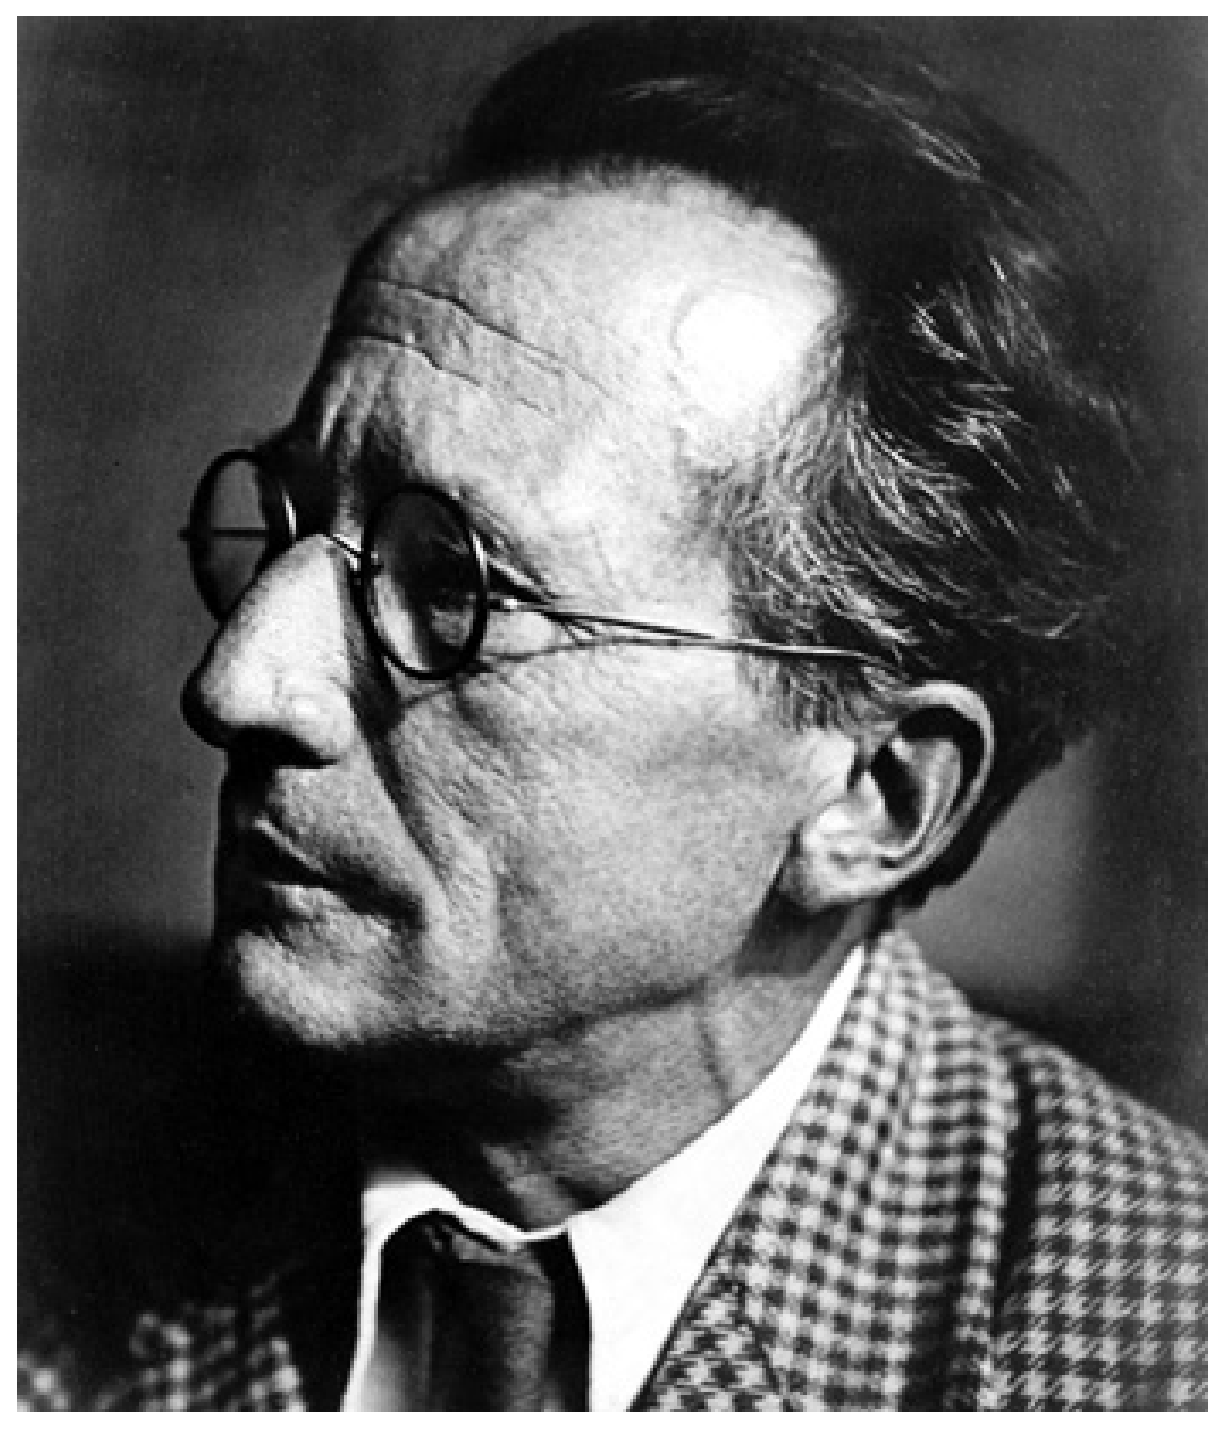
\includegraphics[clip,width=6cm]{SE/schrodinger.ps}
\caption{薛定谔}
\end{center}
\end{figure}

1926年,薛定谔提出波动方程(薛定谔方程)解决了这个问题。

\begin{center}
\begin{equation}\label{schrodinger eq}
    i\hbar \frac{{\partial \Psi }}{{\partial t}} =  - \frac{{\hbar ^2 }}{{2\mu }}\nabla ^2 \Psi  + U(r)\Psi
\end{equation}
\end{center}

薛定谔方程适用范围:

\begin{itemize}
    \item 非相对论情形;
    \item 无粒子的产生和湮灭过程;
\end{itemize}

由于光是相对论的,而且有光子的产生和湮灭,所以薛定谔方程无法描述光子的运动。薛定谔方程也无法描述相对论性电子,
这个问题后来是狄拉克(Paul A.M. Dirac)解决的,狄拉克方程(Dirac
equation)显示,有反粒子(正电子)的存在,因此电子和正电子总是成对产生,成对湮没。

\subsection{薛定谔方程的建立}

\subsubsection{非相对论自由粒子}


现在来考虑一最简单的动力学问题,(1)非相对论的(2)自由的(3)质量为m的单粒子运动。哈密顿量可写为:$H
= p^2/2m$。求解哈密顿方程:

\begin{eqnarray}
\dot x &=& \frac{\partial H}{\partial p} = \frac{p}{m} \\
\dot p &=& \frac{\partial H}{\partial x} = 0
\end{eqnarray}

需要两个初值,即:$x_0$,$p_0$

解出:

\begin{eqnarray}
p &=& p_0 \\
x & = & x_0 + vt = x_0 + \frac{p_0  }{m } t 
\end{eqnarray}

能量:$E = p^2_0 /2m$

这一问题的更直接解法是求解牛顿第二定律(Newton's second
law),即:$F = m \ddot x =- \nabla
V(x)$。这是一个二阶常微分方程,需要两个初值,即:$x_0$和$v_0$。解出来是一条确定的粒子运动轨迹$x(t)$。我们一般说经典力学是一决定性的理论,即只需给定$x_0$和$v_0$(或$p_0$),我们就可以唯一精确地求出粒子运动的轨迹。

\subsubsection{由单色平面波建立}

现在,
我们的任务是求出量子力学版本的``牛顿第二定律''——描述波函数随时间演化的波动方程。这一工作是由薛定谔(E.
Schrodinger)完成的, 因此这个方程就叫薛定谔方程(Schrodinger
equation)。

\begin{equation}
    i\hbar \frac{\partial }{\partial t} \psi = H \psi
\end{equation}

这个式子是普遍形式,不仅对单粒子成立,对多粒子也成立;对相对论量子力学也成立。对单粒子非相对论情形,哈密顿量可写为:$H
= p^2/2m + V(x) = -\frac{\hbar^2}{2m} \nabla^2 +V(x)$
。薛定谔方程是无法由更基本的理论推出的,因此在量子力学的理论体系中被看作是基本假设之一。那么薛定谔方程是如何被猜出来的呢?

对非相对论,自由的单粒子而言,$E=
p^2/2m$,这个等式可否由波函数得出呢?考虑单色平面波$\psi = A e^{i
(px -Et )/ \hbar}$。

\index{Plane wave: 平面波}

$E \psi = i \hbar \frac{\partial }{\partial t}
\psi$,定义能量算符:$\hat E = i \hbar \frac{\partial}{\partial
t}$;由$\hat p = \frac{\hbar}{i} \nabla$,$\frac{p^2}{2m} \psi = -
\frac{\hbar^2}{2m} \nabla^2 \psi$。因此:

\begin{equation}
i \hbar \frac{\partial}{\partial t} \psi = - \frac{\hbar^2}{2m}
\nabla^2 \psi,
\end{equation}

就是$V(x) = 0$(自由情形)时的薛定谔方程。

现在再考虑$V(x) \ne
0$,此时能量($E$)应守恒,只是动能($T$)因势能($V$)的不同而变化。即:波函数的频率($\omega$)不变,但波矢($k$)可变。因此$i
\hbar \frac{\partial }{\partial t} \psi = E \psi =
(-\frac{\hbar^2}{2m} \nabla^2 +V(x)) \psi$。

这样我们就得到了描写非相对论单粒子的薛定谔方程:


\begin{equation}
i\hbar \frac{\partial }{{\partial t}}\psi (x,t) = \left( { -
\frac{{\hbar ^2 }}{{2m}}\nabla ^2  + V(x)} \right)\psi (x,t)
\end{equation}

\index{Schrodinger equation: 薛定谔方程}


这是一个关于时间一阶导数的偏微分方程,因此量子力学是一个决定性的理论(deterministic
theory),只要知道初始时刻的波函数$\psi (x,
t_0)$,由薛定谔方程我们就可求出波函数$\psi(x,t)$随时间的演化\footnote{我们可以定义时间演化算符(time-evolution
operator)$U(t,t_0)$, 使: $\psi(x,t) = U(t,t_0) \psi(x,t_0)$,
这样对波函数的求解就归结为对时间演化算符($U$)的求解。}。

我们一般说量子力学是一概率性理论,
这指的是波函数不直接对应任何物理量(或观测量,observables),
但根据玻恩的统计解释, 我们可由波函数得到物理量的期望值(expectation
value), 即由波函数我们一般不能确切地知道物理量的取值,
我们只能知道物理量各个不同取值的概率分布。在这个意义下,
我们说量子力学是概率的;但就其动力学而言, 量子力学是决定性的。


\subsubsection{由最小作用量原理建立}

薛定谔是利用经典力学的哈密顿理论,加上物质波概念,以氢原子为实例,
建立薛定谔方程的
\footnote{参考:曾谨言 《量子力学 卷II》第98页;金尚年等编《理论力学》第9.3节;}。

为推导简单,我们考虑一维问题:

\index{Principle of least action: 最小作用量原理}

哈密顿量可写为:$H = \frac{{p^2 }}{{2m}} + U(r)$

相应的哈密顿-雅可比方程可写为:$\frac{1}{{2m}}\left( {\nabla S} \right) \cdot \left( {\nabla S} \right) + U(r) = E$, $S$是经典作用量,$S = \int {Ldt} $,拉格朗日:$L=T-V$

薛定谔认为波函数的相位应与经典作用量$S$相当:
$\psi  \sim \exp \left[ {\frac{{iS}}{\hbar }} \right]$

考虑到在量子力学中波函数$\psi $是复函数,我们把哈密顿-雅可比方程重新写为:

\begin{center}
\begin{equation}
 \frac{1}{{2m}}\left( {\nabla S}  \right)^*  \cdot \left( {\nabla S} \right) + U(r) = E
\end{equation}
\end{center}

薛定谔对$S$作了个变换:$S = \frac{\hbar }{i}\ln \psi $,
对两边求偏导:
$\frac{{\partial S}}{{\partial r}} = \frac{\hbar }{{i\psi }}\frac{{\partial \psi }}{{\partial r}}$,
代入哈密顿-雅可比方程:

\begin{center}
$\frac{1}{{2m}}\left( { - \frac{\hbar }{{i\psi ^* }}\frac{{\partial \psi ^* }}{{\partial r}}} \right) \cdot \left( {\frac{\hbar }{{i\psi }}\frac{{\partial \psi }}{{\partial r}}} \right) + U(r) = E$
\end{center}

即:$\frac{{\hbar ^2 }}{{2m}}\left( {\frac{{\partial \psi ^* }}{{\partial r}}} \right) \cdot \left( {\frac{{\partial \psi }}{{\partial r}}} \right) + \left[ {U(r) - E} \right]\psi ^* \psi  = 0$

一般而言,利用最小作用量原理:$\delta S = \delta \int_1^2 {Ldt}  = \delta \int_1^2 {\tilde Ldrdt}  = 0$,可以求出运动方程(这里 $\tilde L$ 表示拉格朗日密度)。
所以构造适合的变分方程就可求出微观粒子运动方程。


薛定谔利用变分条件:

\begin{center}
$\delta \int_1^2 {\left\{ {\frac{{\hbar ^2 }}{{2m}}\left( {\frac{{\partial \psi ^* }}{{\partial r}}} \right) \cdot \left( {\frac{{\partial \psi }}{{\partial r}}} \right) + \left[ {U(r) - E} \right]\psi ^* \psi } \right\}dr}  = 0$
\end{center}

求出了薛定谔方程,但为什么选取这个变分条件,薛定谔并未给出解释。
薛定谔方程是量子力学的基本假定,不能从更基本的假设和定理推出,
所以薛定谔也无法在他的推导中给出变分条件的合理解释。
而薛定谔方程的正确性只有与实验进行比较才能下结论。

变分方程中,把自变量:$\psi ,\psi ^* ,{{\partial \psi } \mathord{\left/
 {\vphantom {{\partial \psi } {\partial x}}} \right.
 \kern-\nulldelimiterspace} {\partial x}},{{\partial \psi ^* } \mathord{\left/
 {\vphantom {{\partial \psi ^* } {\partial r}}} \right.
 \kern-\nulldelimiterspace} {\partial r}}$,看作是广义坐标、广义动量。

所以由欧拉公式:$\frac{d}{{dt}}\frac{{\partial L}}{{\partial \dot q}} - \frac{{\partial L}}{{\partial q}} = 0$(变量对应关系:$t \to r,q \to \psi ^* ,\dot q \to {{\partial \psi ^* } \mathord{\left/
 {\vphantom {{\partial \psi ^* } {\partial r}}} \right.
 \kern-\nulldelimiterspace} {\partial r}}$)

可求出:$\frac{{\hbar ^2 }}{{2m}}\frac{\partial }{{\partial r}}\left( {\frac{{\partial \psi }}{{\partial r}}} \right) - \left[ {U(r) - E} \right]\psi  = 0$,即:

\begin{equation}
E\psi  =  - \frac{{\hbar ^2 }}{{2m}}\frac{{\partial ^2 \psi }}{{\partial r^2 }} + U(r)\psi 
\end{equation}

\subsubsection{多粒子体系的薛定谔方程}

$N$粒子体系能量一般可以表示为:$E = \sum\limits_{i = 1}^N {\frac{{p_i ^2 }}{{2\mu }}}  + U(r_1 ,r_2 ,...,r_N )$

$N$粒子体系波函数可表示为:$\Psi (r_1 ,r_2 ...,r_N )$

动量、能量算子分别写为:

\begin{center}
$E \to i\hbar \frac{\partial }{{\partial t}},p_i  \to  - i\hbar \nabla _i ,\nabla _i  = \vec i\frac{\partial }{{\partial x_i }} + \vec j\frac{\partial }{{\partial y_i }} + \vec k\frac{\partial }{{\partial z_i }}$
\end{center}

所以多粒子体系的薛定谔方程为:

\begin{equation}\label{N particle schordinger}
    i\hbar \frac{\partial }{{\partial t}}\Psi  = \sum\limits_{i = 1}^N {\frac{{\hbar ^2 }}{{2\mu _i }}} \nabla _i ^2 \Psi  + U(r_1 ,r_2 ...,r_N )\Psi
\end{equation}

有了这个方程量子多体问题原则上就解决了,但由于计算的复杂性,这个方程实际上并不实用。
将量子力学(薛定谔方程)应用于各种物理系统,
并发展出适合不同物理系统适用的计算方法和物理概念成为量子力学建立后科学家的主要工作。
如:固体物理实际上就是电子在周期势场(平移对称性)中的求解问题。
现代凝聚态物理学则在此基础上考虑对称破缺,即平移对称性被打破,周期条件不成立。


$U(r_1 ,r_2 ...,r_N )$可作集团展开进行处理,即把多体相互作用化为,单体势、二体势、三体势等求和的形式,
并在此基础上进行近似处理(如:分离变量、重整化等)。

\begin{equation*}
U(r_1 ,r_2 ...,r_N ) = \sum\limits_{i = 1}^N {V(r_i )}  + \frac{1}{2}\sum\limits_{i,j} {V(r_i ,r_j )}  + \frac{1}{{3!}}\sum\limits_{i,j,k} {V(r_i ,r_j ,r_k )}  + ...
\end{equation*}

更重要的是对多粒子体系我们需要考虑交换对称,多粒子体系的波函数$\Psi(..., r_i, ..., r_j , ...)$或者要写为交换对称的形式:

\begin{equation*}
\Psi(..., r_i, ..., r_j , ...) = \Psi(..., r_j, ..., r_i , ...)
\end{equation*}

或者写为交换反对称的形式:

\begin{equation*}
\Psi(..., r_i, ..., r_j , ...) = - \Psi(..., r_j, ..., r_i , ...)
\end{equation*}

前者是所谓玻色子(Boson),玻色子的例子是光子,而后者是所谓费米子(Fermion),费米子的例子是电子。考虑到交换对称,多粒子体系的波函数将会变得十分繁复,但通过引入“产生、湮灭”算符\footnote{有些文献中管这个叫“二次量子化”(second quantization)。},多粒子体系的量子力学问题将重新获得简单清晰的表达。

这些知识我们将留到后面的章节中去介绍。

\subsection{粒子流密度和粒子数守恒}

根据波函数统计解释, 粒子几率密度:$\rho (r,t) = \psi ^* (r,t)\psi
(r,t)$


\index{Statistical interpretation: 统计解释}

\begin{equation}
\frac{{\partial \rho}}{{\partial t}} = \psi ^* \frac{{\partial \psi
}}{{\partial t}} + \frac{{\partial \psi ^* }}{{\partial t}}\psi
\end{equation}

由薛定谔方程:$i\hbar \frac{{\partial \psi }}{{\partial t}} =  - \frac{{\hbar ^2 }}{{2\mu }}\nabla ^2 \psi  + U(r)\psi $,$U(r)$是实函数

所以:

\begin{equation}
\frac{{\partial \psi }}{{\partial t}} = \frac{{i\hbar }}{{2\mu }}\nabla ^2 \psi  + \frac{{U(r)}}{{i\hbar }}\psi ,
\end{equation}

对上式取复共轭:

\begin{equation}
\frac{{\partial \psi ^* }}{{\partial t}} =  - \frac{{i\hbar }}{{2\mu }}\nabla ^2 \psi ^*  - \frac{{U(r)}}{{i\hbar }}\psi ^*
\end{equation}

所以:

\begin{equation}
\frac{{\partial \rho}}{{\partial t}} = \frac{{i\hbar }}{{2\mu
}}\left( {\psi ^* \left( {\nabla ^2 \psi } \right) - \left( {\nabla
^2 \psi ^* } \right)\psi } \right)
\end{equation}

利用:

\begin{eqnarray}
\nabla  \cdot \left[ {\psi ^* \left( {\nabla \psi } \right)} \right] & = & \left( {\nabla \psi ^* } \right) \cdot \left( {\nabla \psi } \right) + \psi ^* \left( {\nabla ^2 \psi } \right) \\
 \nabla  \cdot \left[ {\left( {\nabla \psi ^* } \right)\psi } \right] & = & \left( {\nabla ^2 \psi ^* } \right)\psi  + \left( {\nabla \psi ^* } \right) \cdot \left( {\nabla \psi } \right)
\end{eqnarray}


得到:

\begin{eqnarray*}
\psi ^* \left( {\nabla ^2 \psi } \right) - \left( {\nabla ^2 \psi ^* } \right)\psi  & = & \nabla  \cdot \left[ {\psi ^* \left( {\nabla \psi } \right)} \right] - \nabla  \cdot \left[ {\left( {\nabla \psi ^* } \right)\psi } \right]   \\
{} &  =  &  \nabla  \cdot \left[ {\psi ^* \left( {\nabla \psi } \right) - \left( {\nabla \psi ^* } \right)\psi } \right]
\end{eqnarray*}

所以:

\begin{equation*}
\frac{{\partial \rho}}{{\partial t}} = \frac{{i\hbar }}{{2\mu
}}\left( {\psi ^* \left( {\nabla ^2 \psi } \right) - \left( {\nabla
^2 \psi ^* } \right)\psi } \right) = \frac{{i\hbar }}{{2\mu }}\nabla
\cdot \left[ {\psi ^* \left( {\nabla \psi } \right) - \left( {\nabla
\psi ^* } \right)\psi } \right]
\end{equation*}

定义几率流密度:

\begin{equation}
J =  - \frac{{i\hbar }}{{2\mu }}\left[ {\psi ^* \left( {\nabla \psi } \right) - \left( {\nabla \psi ^* } \right)\psi } \right]
\end{equation}

\index{Probability density flux: 几率流密度}

得到连续性方程:

\begin{equation}\label{continue eq}
    \frac{{\partial \rho}}{{\partial t}} + \nabla  \cdot J = 0
\end{equation}


这个方程也可写为积分形式:

\begin{equation}
\int_V {\frac{{\partial \rho}}{{\partial t}}d\tau  + \oint_S {J \cdot dS} }  = 0.
\end{equation}

即:单位体积增加的几率等于流入单位体积表面几率流之和\footnote{流出为``正'',流入为``负''},几率守恒。

与此类似,我们还可定义:


\begin{description}
    \item[质量流密度] $J_\mu   = \mu J = \frac{{i\hbar }}{2}\left[ {\left( {\nabla \psi ^* } \right)\psi  - \psi ^* \left( {\nabla \psi } \right)} \right]$
    \item[质量守恒定律] $\frac{{\partial \rho_\mu  }}{{\partial t}} + \nabla  \cdot J_\mu   = 0$,($w_\mu   = \mu w$
)
   \end{description}

\begin{description}
    \item[电荷流密度] $J_e  = eJ = \frac{{ie\hbar }}{{2\mu }}\left[ {\left( {\nabla \psi ^* } \right)\psi  - \psi ^* \left( {\nabla \psi } \right)} \right]$
    \item[电荷守恒定律] $\frac{{\partial \rho_e }}{{\partial t}} + \nabla  \cdot J_e  = 0$,($\rho_e  = e\rho$
)
   \end{description}

\index{Probability density: 几率密度}

\textbf{波函数的标准条件:}由于几率密度(Probability
density)和几率流密度应当连续,否则会出现粒子积累效应。
所以波函数应满足三个条件:有限性、连续性、单值性。这三个条件叫波函数的标准条件。

\index{Wave function: 波函数}


\subsection{定态薛定谔方程}

以上讨论的波函数$\psi$都是包含时间变量$t$的,这样的薛定谔方程称为含时薛定谔方程(time
dependent Schrodinger
equation)。如果势($U(r)$)不含时,我们可以用分离变量法(separation
of variables)把含时薛定谔方程化为不含时的薛定谔方程(time
independent Schrodinger equation, 也叫定态薛定谔方程,stationary
Schrodinger equation)。

分离变量:$\psi (r,t) = \psi (r)f(t)$, 得到:

\index{Separation of variables: 分离变量}

\begin{center}
$\frac{{i\hbar }}{f}\frac{{df}}{{dt}} = \frac{1}{\psi }\left[ { - \frac{{\hbar ^2 }}{{2\mu }}\nabla ^2 \psi  + U(r)\psi } \right] = E$
\end{center}

关于$t$的微分方程:

\begin{center}
$\frac{{i\hbar }}{f}\frac{{df}}{{dt}} = E$
\end{center}

其解为:$f(t) = C\exp \left( { - \frac{{iEt}}{\hbar }} \right)$,其中$C$是常数。

关于$r$的微分方程:

\begin{center}
\begin{equation}\label{stationary schordinger eq}
    - \frac{{\hbar ^2 }}{{2\mu }}\nabla ^2 \psi  + U(r)\psi  = E\psi
\end{equation}
\end{center}

\index{Stationary Schrodinger equation: 定态薛定谔方程}

其解为:$\psi (r)$

所以:

\begin{equation}
\psi (r,t) = \psi (r)\exp \left( { - \frac{{iEt}}{\hbar }} \right)
\end{equation}

在这种状态能量具有确定值,所以称为定态,对应波函数称为定态波函数,在定态中几率密度、几率流密度都与时间无关,
公式\ref{stationary schordinger eq}称为定态薛定谔方程(stationary
Schrodinger equation)。

解定态薛定谔方程:$\hat H\psi (r) = E(r)$,可求得波函数:$\psi (r)$

这种类型方程称为本征值方程,$E$称为算符$H$的本征值,对应的$\psi$
称为算符H的本征函数。通过求解能量本征值方程,氢原子的能量只能取分立的数值,
所以能量量子化在薛定谔的理论中是解本征值方程的自然结果,
所以薛定谔认为不应把量子化作为量子力学的基本假设,
他提出薛定谔方程的系列论文题目则是《量子化是本征值问题》。
一般而言,本征值既可能连续,也可能是分立($\left\{ {E_n }
\right\}$)的。

\subsubsection{光学类比}

定态薛定谔方程可以改写为:

\begin{equation}\label{stationaryscheq}
 \nabla^2 \psi + \frac{2m}{\hbar^2} \left[ {E - V(x)} \right] \psi =0
\end{equation}


该式可与光学中的波动方程(wave equation)类比\footnote{参考:D Bohm,
\textbf{Quantum Theory}, pp230},对于单色平面波:$\psi e^{i (kx -
\omega t)}$,代入:$\nabla^2 \vec{A} = \frac{1}{c^2}
\frac{\partial^2 \vec{A}}{\partial t^2}$ 得到:$\nabla^2 \vec{A} = -
\frac{\omega^2}{c^2} \vec{A}$,假设介质的折射率是$n$($n \ge
1$),$c \to \frac{c}{n}$,

得到:

\begin{equation*}
   \nabla^2 \vec{A} + \frac{n^2 \omega^2}{c^2} \vec{A} = 0
\end{equation*}


形式上与定态薛定谔方程\ref{stationaryscheq}相同,$n^2$相当于$\frac{2m
c^2}{\hbar^2 \omega^2} \left[ {E - V(x)}
\right]$。这个类比往往是有用的, 同时我们会发现对$\vec{A}$的求解,
要比对$\psi$复杂,
因为$\vec{A}$对应电场$\vec{E}$和磁场$\vec{B}$共6个分量。



\subsection{克莱因-戈登方程}

在薛定谔提出``单粒子、非相对论薛定谔方程''之前,
狭义相对论对物理学家已经是常识了,
为什么薛定谔不直接提出狭义相对论情形下的波动方程呢?
如果要把``单粒子、非相对论薛定谔方程''推广到相对论情形(具体说是推广到狭义相对论),
我们应该怎么做呢?

比如我们把$E \to i \hbar \frac{\partial}{\partial t}$; $p \to
\frac{\hbar}{i} \nabla$。代入相对论性粒子应满足的能量动量关系: $E^2
= p^2 c^2 + m_0^2 c^4 $,得到:

\begin{center}
\begin{equation}\label{Klein Gordon eq}
    - \hbar ^2 \frac{{\partial ^2 }}{{\partial t^2 }}\psi (r,t) = \left( { - \hbar ^2 c^2 \nabla ^2  + m_0 ^2 c^4 } \right)\psi (r,t)
\end{equation}
\end{center}

\index{Klein-Gordon equation: 克莱因-戈登方程}

这个方程被称为克莱因-戈登方程(Klein-Gordon
equation)。如果把这个方程看作是描写相对论性单粒子的运动方程,
就像普通的薛定谔方程被看作是描写非相对论性单粒子运动的方程,
会碰到如下困难: (1)负几率问题; (2)负能量问题\footnote{参考:L H
Ryder, \textbf{Quantum Field Theory}, 2nd edition, section
2.2}。因此, 克莱因-戈登方程很快就被放弃了。

当$m_0  =
0$时(光子),克莱因-戈登方程退化为Maxwell方程组之一的形式(Maxwell方程组中有电场分量和磁场分量)。
由于Maxwell方程是电磁场方程,不是单个粒子的方程(光强正比于光子数目)。
这启发我们,与薛定谔方程不同,克莱因-戈登方程本质是个场方程,由于其波函数只对应一个分量,
所以克莱因-戈登方程描述了自旋为$0$的场方程。在量子场论中,
克莱因-戈登方程被重新诠释为描述标量场(自旋为$0$)运动的方程,
而粒子在量子场论的语言下则是场的量子。


\subsubsection{几率密度和几率流密度}

对非相对论量子力学而言, 满足薛定谔方程:$i\hbar \frac{\partial
}{\partial t} \psi = [ - \frac{\hbar^2}{2m} \nabla^2 + V]\psi$


定义几率密度:$\rho (x,t) = \psi^*(x,t) \psi(x,t)$,


几率流密度:$\vec{j}(x,t) = - \frac{i \hbar}{2m}[\psi^* \vec{\nabla}
\psi - \psi \vec{\nabla} \psi^*]$

并满足连续性方程:$\frac{\partial \rho}{\partial t} + \nabla \cdot
\vec{j} =0$,第一项为正的话,对应粒子数在$x$附近聚集,
则第二项为负,对应粒子流向$x$附近;即粒子数守恒。非相对论量子力学描述的是一个没有粒子产生和湮灭的粒子数守恒的过程。

如果我们希望把几率密度和几率流密度的定义推广为相对论情形,
需要把$\rho$和$\vec{j}$写成时空对称的形式,因为在狭义相对论中时间和空间取对称的形式。

试把几率密度的定义推广为:

\index{Probability density: 几率密度}

\begin{equation*}
 \rho(x,t) = \frac{i \hbar}{2m}[\psi^* \frac{\partial \psi}{\partial
t} - \psi \frac{\partial \psi^*}{\partial t}]
\end{equation*}


考虑到克莱因-戈登方程包含对时间的二阶导数,$\psi$和$\frac{\partial
\psi}{\partial
t}$在时间$t$可取任意值,这样导致$\rho(x,t)$不再是恒正的,即存在``负几率''。这样表达式$\rho(x,t)
= \frac{i \hbar}{2m}[\psi^* \frac{\partial \psi}{\partial t} - \psi
\frac{\partial \psi^*}{\partial
t}]$就不能被解释为几率密度了,克莱因-戈登方程也不能被理解为一个描述单粒子运动的方程\footnote{L
H Ryder, \textbf{Quantum Field Theory}, pp29}。


\subsection{狄拉克方程}


如果把问题限定为找到一个描述单电子相对论性运动的波动方程,
这个任务是由狄拉克(Paul A.M. Dirac)完成的。
狄拉克的思路是这样的:(1)与薛定谔方程一致只出现对时间$t$的一阶偏导,即写为$i
\hbar \frac{\partial }{\partial t} \psi = H
\psi$的形式;(2)在形式上需要对$(- \hbar^2 c^2 \nabla^2 + m_0^2 c^4
)$ 进行开根运算。

狄拉克通过引入两类矩阵($\alpha_k$和$\beta$)来解决这个开根的问题\footnote{参考:
曾谨言, 《量子力学 II》, 第三版, pp587.}:


左式:$i \hbar \frac{\partial}{\partial t} \psi$ ,右式:$c
\sum_{k=1}^{3} {\alpha_k p_k} + m_0 c^2 \beta$


$\alpha_k$和$\beta$需满足如下关系:


(1)$\alpha_k^2 = I$;(2)$\beta^2 = I$;(3)$\alpha_i \alpha_j +
\alpha_j \alpha_i =0$,$i \ne j$;(4)$\alpha_k \beta + \beta
\alpha_k =0$。


解出来的$\alpha_k$和$\beta$是$4 \times 4$的方阵:


\begin{equation*}
\alpha _k  = \left( {\begin{array}{*{20}c}
   0 & {\sigma _k }  \\
   {\sigma _k } & 0  \\
\end{array}} \right); \beta  = \left( {\begin{array}{*{20}c}
   I & 0  \\
   0 & { - I}  \\
\end{array}} \right)
\end{equation*}


这里的$\sigma$矩阵是描写自旋(spin)运动的泡利矩阵(Pauli
matrix)。最终的狄拉克方程(The Dirac equation)可写作如下形式:


\begin{equation}\label{diracequation}
    \left( {\begin{array}{*{20}c}
   {mc^2 } & {c\sigma  \cdot p}  \\
   {c\sigma  \cdot p} & { - mc^2 }  \\
\end{array}} \right)\left( {\begin{array}{*{20}c}
   {\phi _ +  }  \\
   {\phi _ -  }  \\
\end{array}} \right) = i\hbar \frac{\partial }{{\partial t}}\left( {\begin{array}{*{20}c}
   {\phi _ +  }  \\
   {\phi _ -  }  \\
\end{array}} \right)
\end{equation}


狄拉克方程即可看作是描写单个电子的相对论性运动方程(量子力学),
又可看作是描写二分量(spinor, 自旋为$1/2$)场运动的方程(量子场论)。


\subsection*{练习}

对下列两个定态波函数计算概率流密度:

\begin{eqnarray}
\psi_1 &=& \frac{e^{i k r}}{r} \\
\psi_2 &=& \frac{e^{ - i k r}}{r}
\end{eqnarray}

由所得结果说明$\psi_1$表示的是一个向外传播的球面波,而$\psi_2$表示的是一个向内(即向原点)传播的球面波。


